\documentclass[twoside]{book}

% Packages required by doxygen
\usepackage{calc}
\usepackage{doxygen}
\usepackage{graphicx}
\usepackage[utf8]{inputenc}
\usepackage{makeidx}
\usepackage{multicol}
\usepackage{multirow}
\usepackage{textcomp}
\usepackage[table]{xcolor}

% Font selection
\usepackage[T1]{fontenc}
\usepackage{mathptmx}
\usepackage[scaled=.90]{helvet}
\usepackage{courier}
\usepackage{amssymb}
\usepackage{sectsty}
\renewcommand{\familydefault}{\sfdefault}
\allsectionsfont{%
  \fontseries{bc}\selectfont%
  \color{darkgray}%
}
\renewcommand{\DoxyLabelFont}{%
  \fontseries{bc}\selectfont%
  \color{darkgray}%
}

% Page & text layout
\usepackage{geometry}
\geometry{%
  a4paper,%
  top=2.5cm,%
  bottom=2.5cm,%
  left=2.5cm,%
  right=2.5cm%
}
\tolerance=750
\hfuzz=15pt
\hbadness=750
\setlength{\emergencystretch}{15pt}
\setlength{\parindent}{0cm}
\setlength{\parskip}{0.2cm}
\makeatletter
\renewcommand{\paragraph}{%
  \@startsection{paragraph}{4}{0ex}{-1.0ex}{1.0ex}{%
    \normalfont\normalsize\bfseries\SS@parafont%
  }%
}
\renewcommand{\subparagraph}{%
  \@startsection{subparagraph}{5}{0ex}{-1.0ex}{1.0ex}{%
    \normalfont\normalsize\bfseries\SS@subparafont%
  }%
}
\makeatother

% Headers & footers
\usepackage{fancyhdr}
\pagestyle{fancyplain}
\fancyhead[LE]{\fancyplain{}{\bfseries\thepage}}
\fancyhead[CE]{\fancyplain{}{}}
\fancyhead[RE]{\fancyplain{}{\bfseries\leftmark}}
\fancyhead[LO]{\fancyplain{}{\bfseries\rightmark}}
\fancyhead[CO]{\fancyplain{}{}}
\fancyhead[RO]{\fancyplain{}{\bfseries\thepage}}
\fancyfoot[LE]{\fancyplain{}{}}
\fancyfoot[CE]{\fancyplain{}{}}
\fancyfoot[RE]{\fancyplain{}{\bfseries\scriptsize Generated on Fri Feb 19 2016 14\-:06\-:01 for Arduino Handmade Peripherals functions by Doxygen }}
\fancyfoot[LO]{\fancyplain{}{\bfseries\scriptsize Generated on Fri Feb 19 2016 14\-:06\-:01 for Arduino Handmade Peripherals functions by Doxygen }}
\fancyfoot[CO]{\fancyplain{}{}}
\fancyfoot[RO]{\fancyplain{}{}}
\renewcommand{\footrulewidth}{0.4pt}
\renewcommand{\chaptermark}[1]{%
  \markboth{#1}{}%
}
\renewcommand{\sectionmark}[1]{%
  \markright{\thesection\ #1}%
}

% Indices & bibliography
\usepackage{natbib}
\usepackage[titles]{tocloft}
\setcounter{tocdepth}{3}
\setcounter{secnumdepth}{5}
\makeindex

% Hyperlinks (required, but should be loaded last)
\usepackage{ifpdf}
\ifpdf
  \usepackage[pdftex,pagebackref=true]{hyperref}
\else
  \usepackage[ps2pdf,pagebackref=true]{hyperref}
\fi
\hypersetup{%
  colorlinks=true,%
  linkcolor=blue,%
  citecolor=blue,%
  unicode%
}

% Custom commands
\newcommand{\clearemptydoublepage}{%
  \newpage{\pagestyle{empty}\cleardoublepage}%
}


%===== C O N T E N T S =====

\begin{document}

% Titlepage & ToC
\hypersetup{pageanchor=false}
\pagenumbering{roman}
\begin{titlepage}
\vspace*{7cm}
\begin{center}%
{\Large Arduino Handmade Peripherals functions \\[1ex]\large 0.\-1 }\\
\vspace*{1cm}
{\large Generated by Doxygen 1.8.6}\\
\vspace*{0.5cm}
{\small Fri Feb 19 2016 14:06:01}\\
\end{center}
\end{titlepage}
\clearemptydoublepage
\tableofcontents
\clearemptydoublepage
\pagenumbering{arabic}
\hypersetup{pageanchor=true}

%--- Begin generated contents ---
\chapter{Class Index}
\section{Class List}
Here are the classes, structs, unions and interfaces with brief descriptions\-:\begin{DoxyCompactList}
\item\contentsline{section}{\hyperlink{classport}{port} \\*This contains the attributs and methods for the port driver }{\pageref{df/da6/classport}}{}
\end{DoxyCompactList}

\chapter{File Index}
\section{File List}
Here is a list of all files with brief descriptions\-:\begin{DoxyCompactList}
\item\contentsline{section}{\hyperlink{main_8cpp}{main.\-cpp} }{\pageref{df/d0a/main_8cpp}}{}
\item\contentsline{section}{headers/\hyperlink{ports_8h}{ports.\-h} \\*Class prototype for the ports driver }{\pageref{d2/d54/ports_8h}}{}
\item\contentsline{section}{sources/\hyperlink{ports_8cpp}{ports.\-cpp} }{\pageref{d7/d27/ports_8cpp}}{}
\end{DoxyCompactList}

\chapter{Class Documentation}
\hypertarget{classport}{\section{port Class Reference}
\label{classport}\index{port@{port}}
}


this contains the attributs and methods for the port driver  




{\ttfamily \#include $<$ports.\-h$>$}

\subsection*{Public Member Functions}
\begin{DoxyCompactItemize}
\item 
\hyperlink{classport_ac802d7443286c5e9e5b6b18e6d92b803}{port} (volatile uint8\-\_\-t \&nom)
\begin{DoxyCompactList}\small\item\em Constructor creates a new port instance. \end{DoxyCompactList}\item 
void \hyperlink{classport_ac7a0ac9d9d0c29ddcd6561830a1f848a}{set\-\_\-output} (int pin, bool state)
\begin{DoxyCompactList}\small\item\em sets the pin in D\-I\-G\-I\-T\-A\-L O\-U\-T\-P\-U\-T M\-O\-D\-E \end{DoxyCompactList}\item 
void \hyperlink{classport_a55687ade5fe370dcd855c7b8b6242ceb}{set\-\_\-input} (int pin)
\begin{DoxyCompactList}\small\item\em sets the pin as I\-N\-P\-U\-T M\-O\-D\-E with pull-\/up disable \end{DoxyCompactList}\item 
void \hyperlink{classport_aa0d4a6e02cc7610e5f50a9aa0e1654c2}{invert} (const int \&time)
\begin{DoxyCompactList}\small\item\em inverts the state of the specified P\-O\-R\-T (D\-E\-F\-A\-U\-L\-T S\-T\-A\-T\-E\-: 10101010) \end{DoxyCompactList}\end{DoxyCompactItemize}
\subsection*{Protected Attributes}
\begin{DoxyCompactItemize}
\item 
volatile uint8\-\_\-t $\ast$ \hyperlink{classport_a7d360768f8ba1c3f2c65c0c72bafaf54}{port\-\_\-name}
\begin{DoxyCompactList}\small\item\em pointer to the io register P\-O\-R\-Tx (x\{B,C,D\}) \end{DoxyCompactList}\item 
bool \hyperlink{classport_a296e1dfa3d9c7e5b8fa707355a523f6c}{broche}
\begin{DoxyCompactList}\small\item\em ensure the creation of a port instance \end{DoxyCompactList}\end{DoxyCompactItemize}


\subsection{Detailed Description}
this contains the attributs and methods for the port driver 

Definition at line 20 of file ports.\-h.



\subsection{Constructor \& Destructor Documentation}
\hypertarget{classport_ac802d7443286c5e9e5b6b18e6d92b803}{\index{port@{port}!port@{port}}
\index{port@{port}!port@{port}}
\subsubsection[{port}]{\setlength{\rightskip}{0pt plus 5cm}port\-::port (
\begin{DoxyParamCaption}
\item[{volatile uint8\-\_\-t \&}]{nom}
\end{DoxyParamCaption}
)}}\label{classport_ac802d7443286c5e9e5b6b18e6d92b803}


Constructor creates a new port instance. 


\begin{DoxyParams}{Parameters}
{\em \&nom} & the name of the port (P\-O\-R\-T\-B,P\-O\-R\-T\-C,P\-O\-R\-T\-D) \\
\hline
\end{DoxyParams}
\begin{DoxyReturn}{Returns}
nothing 
\end{DoxyReturn}


Definition at line 19 of file ports.\-cpp.



\subsection{Member Function Documentation}
\hypertarget{classport_aa0d4a6e02cc7610e5f50a9aa0e1654c2}{\index{port@{port}!invert@{invert}}
\index{invert@{invert}!port@{port}}
\subsubsection[{invert}]{\setlength{\rightskip}{0pt plus 5cm}void port\-::invert (
\begin{DoxyParamCaption}
\item[{const int \&}]{time}
\end{DoxyParamCaption}
)}}\label{classport_aa0d4a6e02cc7610e5f50a9aa0e1654c2}


inverts the state of the specified P\-O\-R\-T (D\-E\-F\-A\-U\-L\-T S\-T\-A\-T\-E\-: 10101010) 


\begin{DoxyParams}{Parameters}
{\em time} & gives the time between each state (in miliseconds) \\
\hline
\end{DoxyParams}
\begin{DoxyReturn}{Returns}
nothing 
\end{DoxyReturn}


Definition at line 113 of file ports.\-cpp.

\hypertarget{classport_a55687ade5fe370dcd855c7b8b6242ceb}{\index{port@{port}!set\-\_\-input@{set\-\_\-input}}
\index{set\-\_\-input@{set\-\_\-input}!port@{port}}
\subsubsection[{set\-\_\-input}]{\setlength{\rightskip}{0pt plus 5cm}void port\-::set\-\_\-input (
\begin{DoxyParamCaption}
\item[{int}]{pin}
\end{DoxyParamCaption}
)}}\label{classport_a55687ade5fe370dcd855c7b8b6242ceb}


sets the pin as I\-N\-P\-U\-T M\-O\-D\-E with pull-\/up disable 


\begin{DoxyParams}{Parameters}
{\em pin} & the pin number of the port (P\-I\-N0..P\-I\-N7) \\
\hline
\end{DoxyParams}
\begin{DoxyReturn}{Returns}
nothing 
\end{DoxyReturn}


Definition at line 74 of file ports.\-cpp.

\hypertarget{classport_ac7a0ac9d9d0c29ddcd6561830a1f848a}{\index{port@{port}!set\-\_\-output@{set\-\_\-output}}
\index{set\-\_\-output@{set\-\_\-output}!port@{port}}
\subsubsection[{set\-\_\-output}]{\setlength{\rightskip}{0pt plus 5cm}void port\-::set\-\_\-output (
\begin{DoxyParamCaption}
\item[{int}]{pin, }
\item[{bool}]{state}
\end{DoxyParamCaption}
)}}\label{classport_ac7a0ac9d9d0c29ddcd6561830a1f848a}


sets the pin in D\-I\-G\-I\-T\-A\-L O\-U\-T\-P\-U\-T M\-O\-D\-E 


\begin{DoxyParams}{Parameters}
{\em pin} & the pin number of the port (P\-I\-N0..P\-I\-N7) \\
\hline
{\em state} & the pin state (H\-I\-G\-H or L\-O\-W) \\
\hline
\end{DoxyParams}
\begin{DoxyReturn}{Returns}
nothing 
\end{DoxyReturn}


Definition at line 23 of file ports.\-cpp.



\subsection{Member Data Documentation}
\hypertarget{classport_a296e1dfa3d9c7e5b8fa707355a523f6c}{\index{port@{port}!broche@{broche}}
\index{broche@{broche}!port@{port}}
\subsubsection[{broche}]{\setlength{\rightskip}{0pt plus 5cm}bool port\-::broche\hspace{0.3cm}{\ttfamily [protected]}}}\label{classport_a296e1dfa3d9c7e5b8fa707355a523f6c}


ensure the creation of a port instance 



Definition at line 67 of file ports.\-h.

\hypertarget{classport_a7d360768f8ba1c3f2c65c0c72bafaf54}{\index{port@{port}!port\-\_\-name@{port\-\_\-name}}
\index{port\-\_\-name@{port\-\_\-name}!port@{port}}
\subsubsection[{port\-\_\-name}]{\setlength{\rightskip}{0pt plus 5cm}volatile uint8\-\_\-t$\ast$ port\-::port\-\_\-name\hspace{0.3cm}{\ttfamily [protected]}}}\label{classport_a7d360768f8ba1c3f2c65c0c72bafaf54}


pointer to the io register P\-O\-R\-Tx (x\{B,C,D\}) 



Definition at line 66 of file ports.\-h.



The documentation for this class was generated from the following files\-:\begin{DoxyCompactItemize}
\item 
headers/\hyperlink{ports_8h}{ports.\-h}\item 
sources/\hyperlink{ports_8cpp}{ports.\-cpp}\end{DoxyCompactItemize}

\chapter{File Documentation}
\hypertarget{ports_8h}{\section{headers/ports.h File Reference}
\label{ports_8h}\index{headers/ports.\-h@{headers/ports.\-h}}
}


Class prototype for the ports driver.  


This graph shows which files directly or indirectly include this file\-:\nopagebreak
\begin{figure}[H]
\begin{center}
\leavevmode
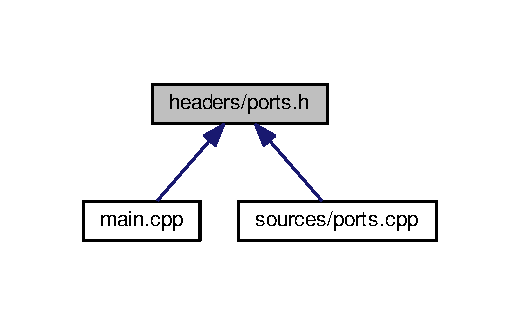
\includegraphics[width=249pt]{d2/d08/ports_8h__dep__incl}
\end{center}
\end{figure}
\subsection*{Classes}
\begin{DoxyCompactItemize}
\item 
class \hyperlink{classport}{port}
\begin{DoxyCompactList}\small\item\em this contains the attributs and methods for the port driver \end{DoxyCompactList}\end{DoxyCompactItemize}


\subsection{Detailed Description}
Class prototype for the ports driver. This contains the class for the ports driver and also the attributs and methods you will need

\begin{DoxyAuthor}{Author}
Alex velásquez Meling  No known bugs 
\end{DoxyAuthor}


Definition in file \hyperlink{ports_8h_source}{ports.\-h}.


\hypertarget{main_8cpp}{\section{main.\-cpp File Reference}
\label{main_8cpp}\index{main.\-cpp@{main.\-cpp}}
}
{\ttfamily \#include $<$avr/io.\-h$>$}\\*
{\ttfamily \#include $<$stdio.\-h$>$}\\*
{\ttfamily \#include $<$util/delay\-\_\-basic.\-h$>$}\\*
{\ttfamily \#include \char`\"{}headers/ports.\-h\char`\"{}}\\*
Include dependency graph for main.\-cpp\-:\nopagebreak
\begin{figure}[H]
\begin{center}
\leavevmode
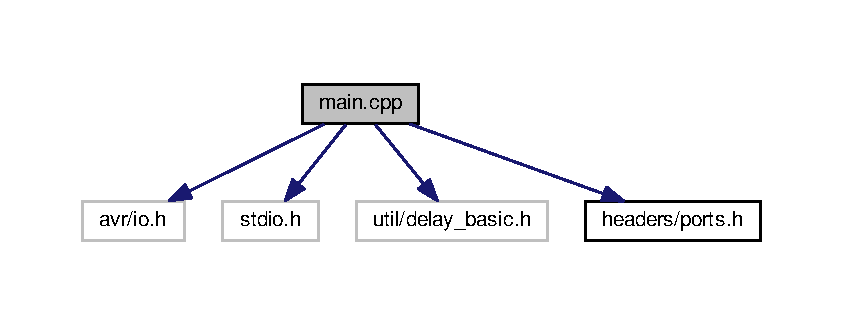
\includegraphics[width=350pt]{da/dce/main_8cpp__incl}
\end{center}
\end{figure}
\subsection*{Macros}
\begin{DoxyCompactItemize}
\item 
\#define \hyperlink{main_8cpp_a5bb885982ff66a2e0a0a45a8ee9c35e2}{H\-I\-G\-H}~true
\item 
\#define \hyperlink{main_8cpp_ab811d8c6ff3a505312d3276590444289}{L\-O\-W}~false
\item 
\#define \hyperlink{main_8cpp_a4c601b4f90966724c2de786d8bd9eb82}{low}~\hyperlink{main_8cpp_ab811d8c6ff3a505312d3276590444289}{L\-O\-W}
\item 
\#define \hyperlink{main_8cpp_a9ce2716323ceb0e2133340a161f33a6c}{high}~\hyperlink{main_8cpp_a5bb885982ff66a2e0a0a45a8ee9c35e2}{H\-I\-G\-H}
\end{DoxyCompactItemize}
\subsection*{Functions}
\begin{DoxyCompactItemize}
\item 
int \hyperlink{main_8cpp_a840291bc02cba5474a4cb46a9b9566fe}{main} (void)
\end{DoxyCompactItemize}


\subsection{Macro Definition Documentation}
\hypertarget{main_8cpp_a5bb885982ff66a2e0a0a45a8ee9c35e2}{\index{main.\-cpp@{main.\-cpp}!H\-I\-G\-H@{H\-I\-G\-H}}
\index{H\-I\-G\-H@{H\-I\-G\-H}!main.cpp@{main.\-cpp}}
\subsubsection[{H\-I\-G\-H}]{\setlength{\rightskip}{0pt plus 5cm}\#define H\-I\-G\-H~true}}\label{main_8cpp_a5bb885982ff66a2e0a0a45a8ee9c35e2}


Definition at line 6 of file main.\-cpp.

\hypertarget{main_8cpp_a9ce2716323ceb0e2133340a161f33a6c}{\index{main.\-cpp@{main.\-cpp}!high@{high}}
\index{high@{high}!main.cpp@{main.\-cpp}}
\subsubsection[{high}]{\setlength{\rightskip}{0pt plus 5cm}\#define high~{\bf H\-I\-G\-H}}}\label{main_8cpp_a9ce2716323ceb0e2133340a161f33a6c}


Definition at line 9 of file main.\-cpp.

\hypertarget{main_8cpp_ab811d8c6ff3a505312d3276590444289}{\index{main.\-cpp@{main.\-cpp}!L\-O\-W@{L\-O\-W}}
\index{L\-O\-W@{L\-O\-W}!main.cpp@{main.\-cpp}}
\subsubsection[{L\-O\-W}]{\setlength{\rightskip}{0pt plus 5cm}\#define L\-O\-W~false}}\label{main_8cpp_ab811d8c6ff3a505312d3276590444289}


Definition at line 7 of file main.\-cpp.

\hypertarget{main_8cpp_a4c601b4f90966724c2de786d8bd9eb82}{\index{main.\-cpp@{main.\-cpp}!low@{low}}
\index{low@{low}!main.cpp@{main.\-cpp}}
\subsubsection[{low}]{\setlength{\rightskip}{0pt plus 5cm}\#define low~{\bf L\-O\-W}}}\label{main_8cpp_a4c601b4f90966724c2de786d8bd9eb82}


Definition at line 8 of file main.\-cpp.



\subsection{Function Documentation}
\hypertarget{main_8cpp_a840291bc02cba5474a4cb46a9b9566fe}{\index{main.\-cpp@{main.\-cpp}!main@{main}}
\index{main@{main}!main.cpp@{main.\-cpp}}
\subsubsection[{main}]{\setlength{\rightskip}{0pt plus 5cm}int main (
\begin{DoxyParamCaption}
\item[{void}]{}
\end{DoxyParamCaption}
)}}\label{main_8cpp_a840291bc02cba5474a4cb46a9b9566fe}


Definition at line 12 of file main.\-cpp.


\hypertarget{ports_8cpp}{\section{sources/ports.cpp File Reference}
\label{ports_8cpp}\index{sources/ports.\-cpp@{sources/ports.\-cpp}}
}
{\ttfamily \#include $<$stdio.\-h$>$}\\*
{\ttfamily \#include $<$avr/io.\-h$>$}\\*
{\ttfamily \#include $<$util/delay.\-h$>$}\\*
{\ttfamily \#include \char`\"{}../headers/ports.\-h\char`\"{}}\\*
Include dependency graph for ports.\-cpp\-:\nopagebreak
\begin{figure}[H]
\begin{center}
\leavevmode
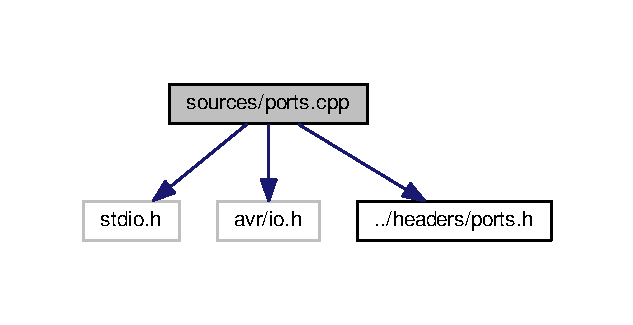
\includegraphics[width=350pt]{d7/d97/ports_8cpp__incl}
\end{center}
\end{figure}

%--- End generated contents ---

% Index
\newpage
\phantomsection
\addcontentsline{toc}{chapter}{Index}
\printindex

\end{document}
